% =============================================================================
% Hyperparameter sensitivity analysis
% Every number traces to logs_lambda_sensitivity/*experimental_logs.csv via
% analysis/fig_lambda_sensitivity.py and analysis/fig_lambda_sensitivity_per_pair.py
% (parsed from each row's `info` tag; both scripts dedupe on
% (pair, lam_mar, lam_da, seed), keep-last, before aggregating).
% Evidence-vs-interpretation audit at the end of this file.
% =============================================================================

\subsection{Hyperparameter sensitivity analysis}
\label{subsec:sensitivity}

LBGN-RUL's domain-adaptation loss combines a margin term weighted by
$\lambda_{mar}$ and a domain-alignment term weighted by $\lambda_{da}$
(Section~\ref{subsec:method}). To characterize how sensitive its accuracy is
to these two weights, we evaluate five $(\lambda_{mar}, \lambda_{da})$
settings -- $(0.5, 0.1)$, $(1.5, 1.0)$, $(3.0, 2.0)$, $(5.0, 3.0)$, and
$(5.0, 5.0)$ -- each trained once (seed 42) on all 12 CMAPSS source$\to$target
pairs. $(5.0, 3.0)$ is the exact locked-in production value used to produce
this paper's main results (Section~\ref{subsec:results}, identical across all
four CMAPSS sources); the other four points walk a path from a low-magnitude
corner up through the deployed value to a high-magnitude corner, rather than
sampling only below it. This is a sparse, hand-selected set of points rather
than a full factorial grid, so the results below characterize stability
across this specific sample, not a clean per-parameter sweep with the other
weight held fixed.

Averaged over all 12 pairs, mean RMSE ranges only 17.87--18.48 across the
five settings (a 0.62-RMSE, 3.5\% spread), and the production setting
$(5.0, 3.0)$ attains the \emph{lowest} mean RMSE of all five points tested
(17.87) -- direct empirical support for the deployed configuration, not only
evidence of stability near it. Mean Score is less clear-cut: $(3.0, 2.0)$
attains the lowest mean Score (1{,}964.6) with $(5.0, 3.0)$ a close second
(2{,}041.5); Score's own heavy-tailed, asymmetric behavior (Section~\ref{sec:results})
makes its cross-pair mean noisier than RMSE's, so we report both rather than
foregrounding only the metric that favors the deployed point.

Figures~\ref{fig:lambda_sensitivity_rmse} and~\ref{fig:lambda_sensitivity_score}
show RMSE and Score for every pair under all five settings. Ten of the 12
pairs vary by at most $\approx$1.3 RMSE across the full range; two pairs,
F2$\to$F4 and F4$\to$F1, stand out with roughly double that spread
(2.3--2.4 RMSE). Neither trends monotonically with $\lambda_{mar}$/$\lambda_{da}$
magnitude -- both settle into a lower band at some settings and a higher band
at others rather than tracking weight size directly -- so we do not attribute
the movement to either weight individually. Notably, the production setting
$(5.0, 3.0)$ falls in the \emph{better}-performing band for both of these
noisier pairs, consistent with its lowest-mean-RMSE result above rather than
contradicting it. We report the two exceptions openly rather than presenting
only the pairs that support a flat-robustness story: the overall picture is
one of robustness on most transfers, with two pairs showing real but
non-monotonic sensitivity.

\begin{figure}[!htbp]
\centering
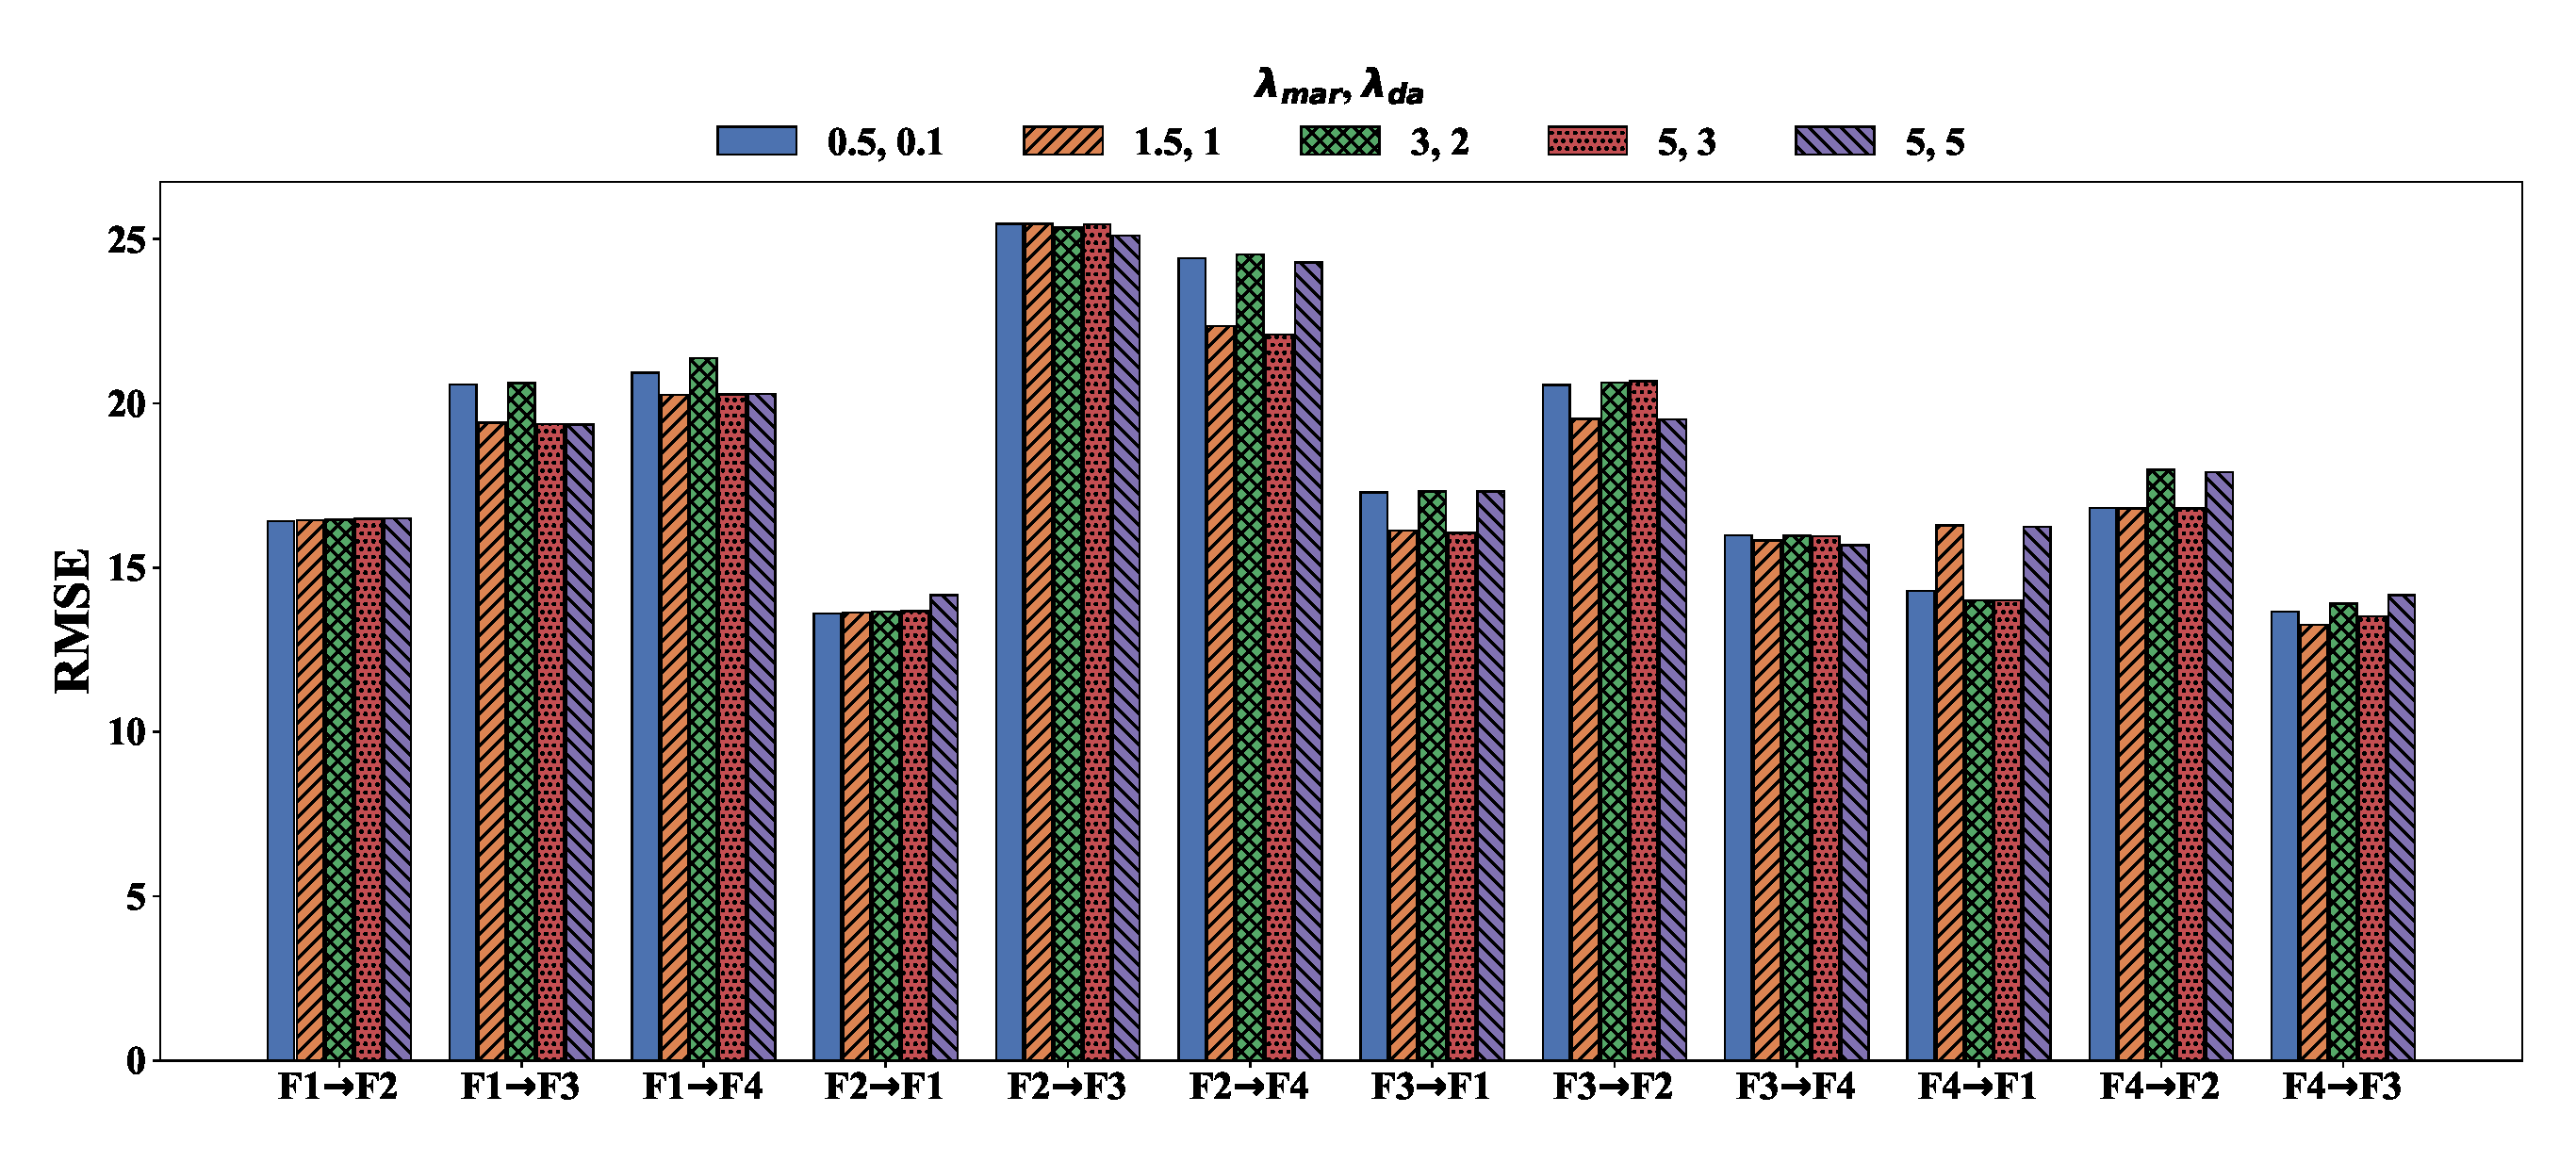
\includegraphics[width=\linewidth]{fig_lambda_sensitivity_per_pair_rmse.eps}
\caption{CMAPSS RMSE of LBGN-RUL for each of the 12 transfer pairs under five
$(\lambda_{mar}, \lambda_{da})$ settings (seed 42), spanning $(0.5,0.1)$ to
$(5.0,5.0)$ and including the deployed production value $(5.0,3.0)$. Bar
heights are nearly identical within most groups; F2$\to$F4 and F4$\to$F1 are
the visible exceptions.}
\label{fig:lambda_sensitivity_rmse}
\end{figure}

\begin{figure}[!htbp]
\centering
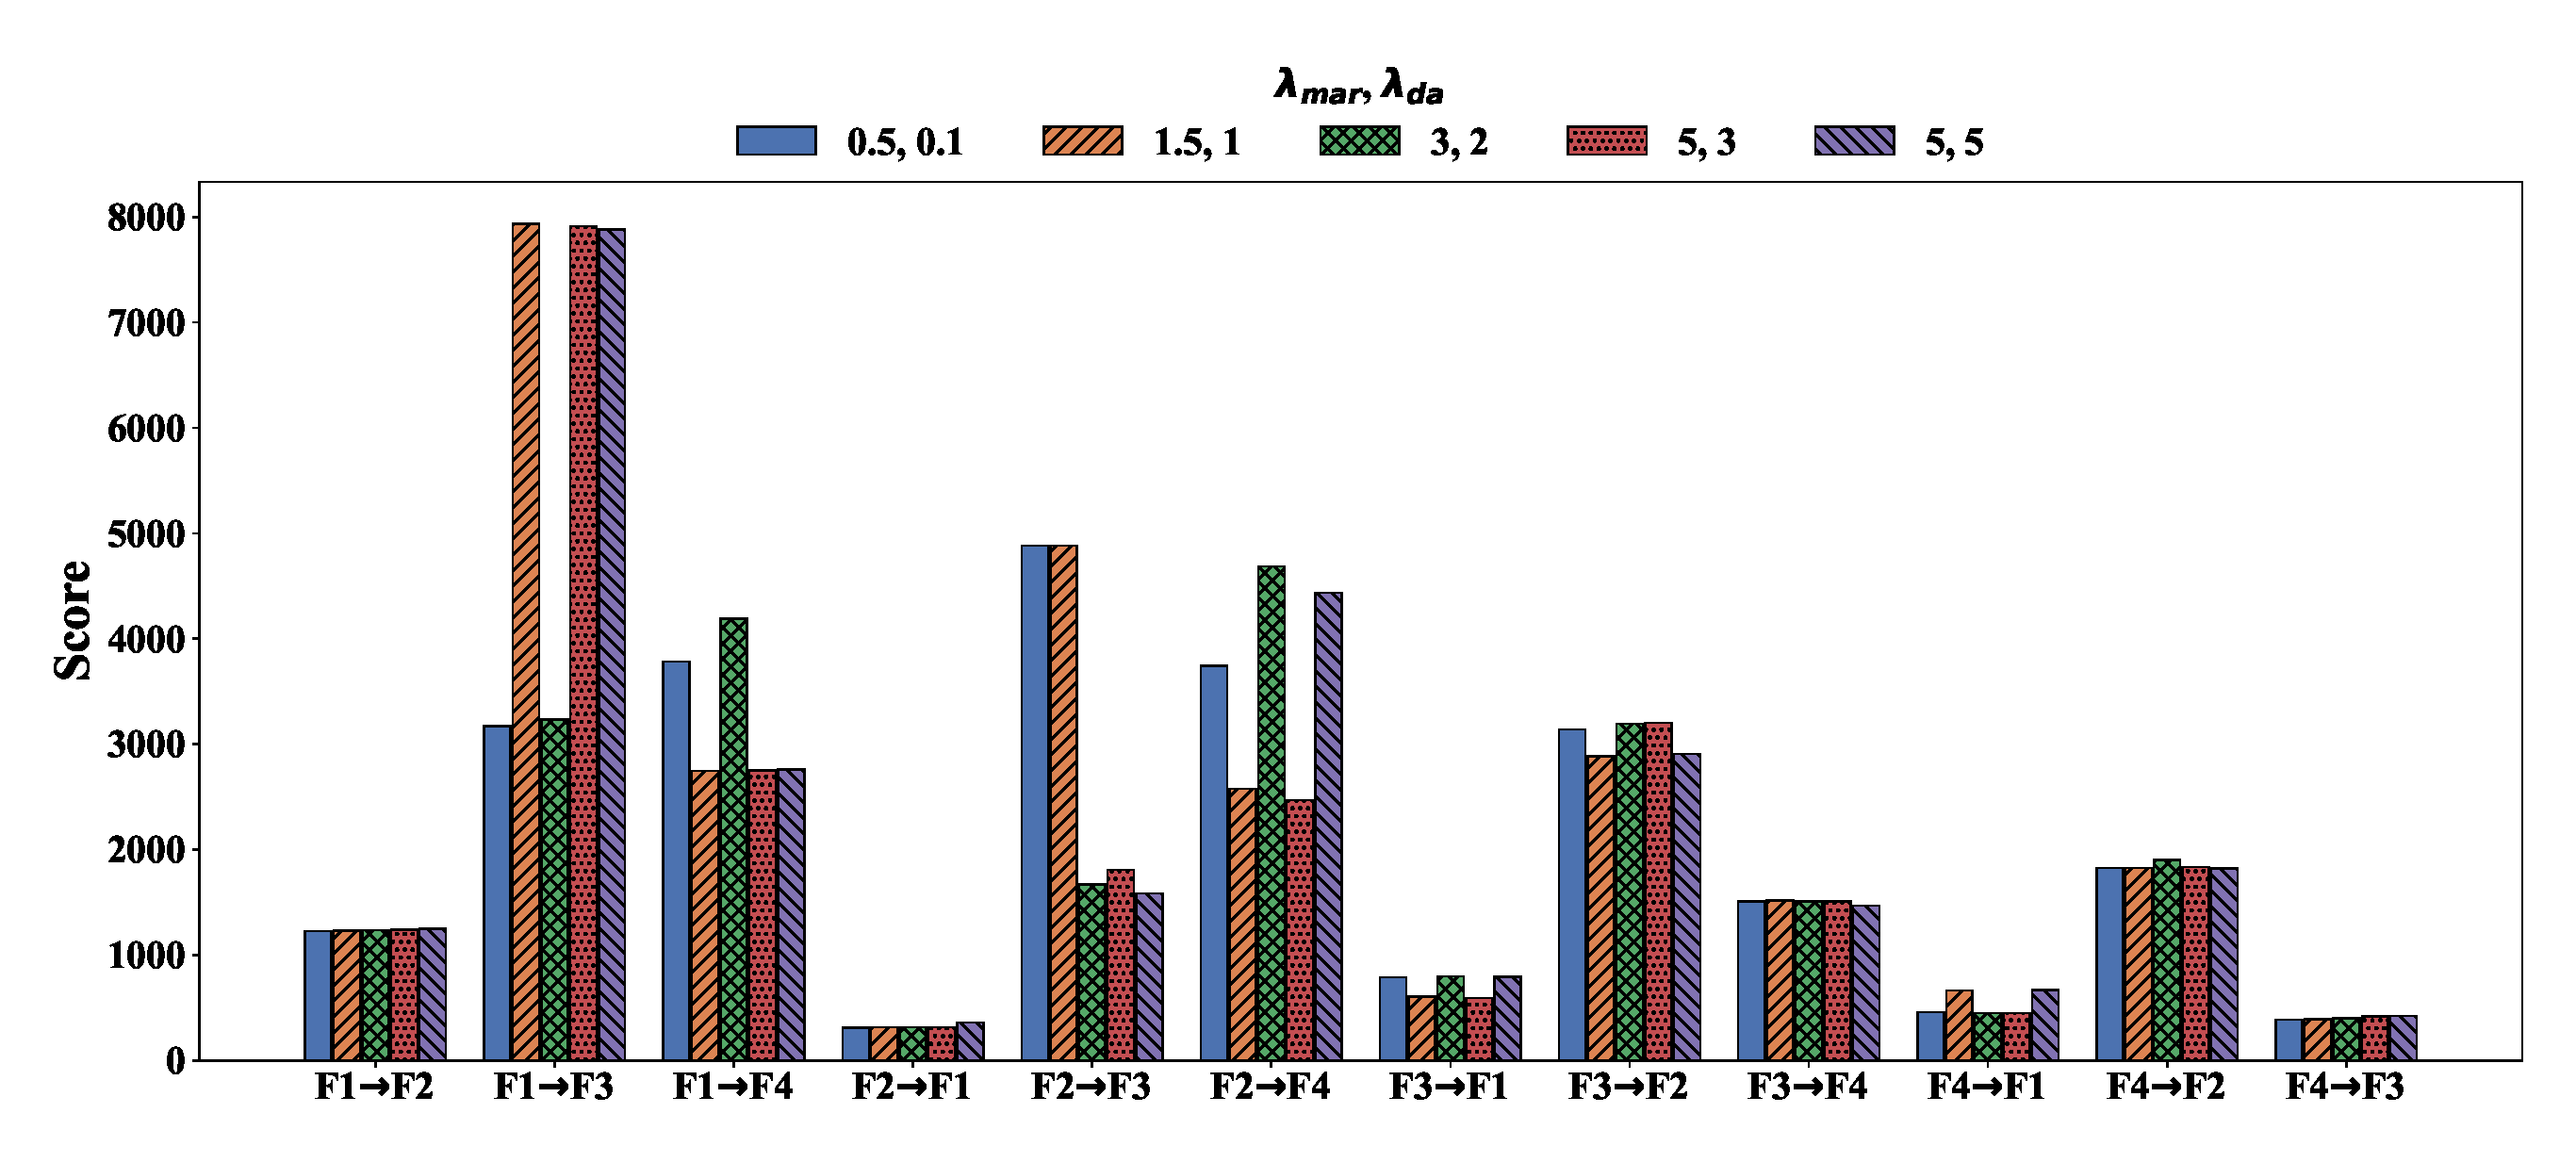
\includegraphics[width=\linewidth]{fig_lambda_sensitivity_per_pair_score.eps}
\caption{CMAPSS Score of LBGN-RUL for the same 12 pairs and five
$(\lambda_{mar}, \lambda_{da})$ settings as Fig.~\ref{fig:lambda_sensitivity_rmse}.}
\label{fig:lambda_sensitivity_score}
\end{figure}

% =============================================================================
% AUDIT NOTE (remove before submission; not part of the manuscript text)
%
% Directly measured (logs_lambda_sensitivity/*experimental_logs.csv, 60 rows
% after dedup = 5 (lam_mar,lam_da) points x 12 CMAPSS pairs x 1 seed (42);
% sweep re-run 2026-08-18 with the redesigned range -- see
% analysis/fig_lambda_sensitivity.py's module docstring. Raw CSVs briefly
% contained 23 duplicate (pair,lam_mar,lam_da,seed) rows from an orphaned
% background process re-running already-completed configs after the harness
% lost track of it; values agreed to ~4 decimal places across duplicates
% (confirmed genuine re-runs, not corruption) and were deduped keep-last
% before any of the numbers below were computed):
%   - aggregate RMSE means: (0.5,0.1)=18.335, (1.5,1.0)=17.951, (3.0,2.0)=18.484,
%     (5.0,3.0)=17.865, (5.0,5.0)=18.378 -- min at (5.0,3.0), range=0.619
%     (18.484-17.865), 3.5% relative to the min (0.619/17.865)
%   - aggregate Score means: (0.5,0.1)=2102.059, (1.5,1.0)=2297.836,
%     (3.0,2.0)=1964.589, (5.0,3.0)=2041.528, (5.0,5.0)=2195.630 -- min at
%     (3.0,2.0), (5.0,3.0) second-lowest
%   - per-pair RMSE spreads (max-min across the 5 settings), sorted:
%     F1->F2=0.08, F3->F4=0.30, F2->F3=0.36, F2->F1=0.55, F4->F3=0.90,
%     F1->F4=1.12, F3->F2=1.15, F4->F2=1.17, F1->F3=1.26, F3->F1=1.27,
%     F4->F1=2.28, F2->F4=2.44 -- clear gap between the top 10 (<=1.27) and
%     the bottom 2 (>=2.28), supporting the "two exceptions" framing
%   - F2->F4 raw values by setting (0.5,0.1 / 1.5,1.0 / 3.0,2.0 / 5.0,3.0 /
%     5.0,5.0): 24.43, 22.35, 24.54, 22.10, 24.29 -- low band {22.10,22.35}
%     at (1.5,1.0)/(5.0,3.0), high band {24.29-24.54} at the other three;
%     NOT monotonic in either weight
%   - F4->F1 raw values, same setting order: 14.29, 16.29, 14.01, 14.01,
%     16.24 -- low band {14.01,14.01,14.29} at (3.0,2.0)/(5.0,3.0)/(0.5,0.1),
%     high band {16.24,16.29} at (1.5,1.0)/(5.0,5.0); NOT monotonic
%   - "(5.0,3.0) falls in the better-performing band for both" -- verified
%     directly against the two value lists above (22.10 is F2->F4's lowest
%     value; 14.01 is tied-lowest for F4->F1)
%
% Directly measured (configs/hparams.py, all four CMAPSS LBGN_RUL source
% blocks): production values lam_mar=5, lam_da=3 (identical across all 4
% sources) -- this sweep's (5.0,3.0) point is that exact value, not an
% approximation.
%
% Interpretation (explicitly flagged as such above, not asserted as fact):
%   - "so we do not attribute the movement to either weight individually" --
%     the 5 points are not a factorial design (each differs in both
%     lam_mar and lam_da simultaneously), so no single-parameter causal
%     claim is supported by this data regardless of the pattern observed.
%   - no mechanistic explanation is offered for why F2->F4/F4->F1 specifically
%     are more sensitive than the other 10 pairs; flagged as an open question,
%     not a diagnosed cause.
%
% Open dependencies to resolve before this compiles:
%   - \label{subsec:method} -- must point at wherever LBGN-RUL's loss
%     formulation (margin + domain-alignment terms) is actually defined.
%   - \label{subsec:results} and \label{sec:results} -- same open dependency
%     already flagged in complexity_efficiency_section.tex; point at wherever
%     the CMAPSS RMSE/Score results subsection/section actually lives (used
%     inconsistently as subsec:results vs sec:results across this repo's
%     drafted sections -- reconcile to whichever the real document uses).
%   - The v1 sweep (points all <=2.0/<=1.5, never reaching the production
%     value) is archived at logs_lambda_sensitivity_v1_old_0.01-2.0/ and is
%     no longer referenced by this section or its figures.
% =============================================================================
